\section{Objectifs}
Les objectifs de ce projet sont de développer un système de prédiction de stratégie de course en temps réel pour les équipes de course, basé sur l'analyse des données de la voiture et des conditions de la piste, et de fournir des recommandations pour optimiser les temps de tour et les arrêts aux stands.
\subsection{Objectifs fondamentaux}
\begin{itemize}
    \item Implémenter un pipeline de traitement et d’analyse de données avec des algorithmes de Machine Learning pour recommander l’entrée au stand d’une voiture en fonction de la situation de course.
    \item Établir un dataset adéquat à l’entrainement d’un tel modèle à partir de multiples sources de données brutes.
    \item Fournir des prédictions réalistes et interprétables par les experts métiers.
    \item Le système est réactif et permet des prédictions rapides (moins de 30 secondes).
\end{itemize}
\subsection{Objectifs optionnels}
\begin{itemize}
    \item Développer une interface utilisateur pour facilement accéder aux recommandations stratégiques.
    \item Étendre le modèle pour les conditions météorologiques incertaines comme les chutes de pluie.
\end{itemize}

\section{Principe de la stratégie en Formule 1}
L'objectif fondamental de la stratégie est de minimiser le temps que l'on prend pour finir tous les tours de course.
En formule 1, les écuries doivent choisir entre 3 composés de pneumatique à utiliser.
Ces composés nommés tendres, mediums et durs performent différemment le long de la course, les plus tendres offrant une meilleure adhérence, mais s'usant plus rapidement.

Pour illustrer cette section on a simulé en python une course très simplifiée. La simulation considère que la voiture est seule sur la piste,
qu'il n'y a pas de variation dans la performance du pilote ou dans l'état du circuit.
La course est discrétisée en $N$ tours où chaque temps au tour $t_{tour}$ est défini comme montré dans l'équation \ref{eq:tour} :

\begin{equation} \label{eq:tour}
    \begin{split}
        t_{tour}=t_{optimal} + t_{carburant} + t_{pneu}
    \end{split}
\end{equation}

$t_{optimal}$ est le temps optimal que la voiture peut faire sur le circuit dans les meilleures conditions.
$t_{carburant}$ est le temps perdu en raison du poids du carburant embarqué. Au fil de la course ce temps s'amoindrit lorsque que
le carburant est consommé. $t_{carburant}$ est calculé comme l'équation \ref{eq:carburant}.
Où $t_{penalite}$ est le temps au tour perdu par kg. Cette valeur dépend du circuit, mais est approximable à 0.03 seconde pour les circuits de longueur moyenne. \cite{royalAcademyOfEngineering} \cite{hurryUpAndWeight}
$p_{depart}$ est la quantité en kg de carburant au départ de la course, pour cette simulation, nous faisons l'hypothèse que la voiture commence avec le maximum de carburant autorisé, c'est-à-dire 110 kg.
$p_{consomme}$ est la quantité de carburant en kg qui est consommé en 1 tour de course, elle est calculée en estimant que la consommation de carburant est constante, soit $\frac{p_{depart}}{N}$.
$n$ est le nombre de tours parcourus jusqu'à maintenant.

\begin{equation} \label{eq:carburant}
    \begin{split}
        t_{carburant} = t_{penalite} * (p_{depart} - p_{consomme} * n)
    \end{split}
\end{equation}

$t_{pneu}$ est le temps perdu en raison de l'adhérence des pneumatiques, elle dépend du composé et de la dégradation du pneu. Le détail est donné dans l'équation \ref{eq:pneu},
elle approxime la dégradation des pneus par la formule de calcul des intérêts composés pour représenter la chute de performance que l'on peut observer avec les pneumatiques \cite{parttimeanalyst}.
$t_{per\textit{f}ormance}$ est le temps perdu comparé à la performance du pneu le plus tendre.
Le taux de dégradation du pneu par tour, exprimé en pourcentage par $d$ et le $\delta{d}$ l'augmentation de ce taux par tour.

\begin{equation} \label{eq:pneu}
    \begin{split}
        t_{pneu} = t_{per\textit{f}ormance} + d * (1 + \delta{d}) ^{(n - 1)}
    \end{split}
\end{equation}

La figure \ref{Comparaison de la dégradation} illustre l'influence de la dégradation sur la performance des différents composés de pneu utilisant
la simulation avec des paramètres trouvable dans la table \ref{Paramètres de la simulation} en annexe.
Les pneus tendres sont plus performant initialement avant de rapidement perdre en performance, le même phénomène se produit avec les mediums et les durs, mais après un plus grand laps de temps.
Cette différence en performance entre les composés dépend du circuit et est difficile à estimer précisément en amont de la course.

\fig[H, width=0.9\textwidth]{\label{Comparaison de la dégradation}Comparaison de la dégradation des différents composés de pneu}{compounds_comparison.svg}

Les temps au tour sont successivement additionnés pour obtenir la variable $t_{course}$, qui représente la durée totale d'une stratégie simulée comme présenté dans l'équation \ref{eq:course}.
\begin{equation} \label{eq:course}
    \begin{split}
        t_{course} = \sum_{i=1}^{N}{t_{tour}(i)}
    \end{split}
\end{equation}

On peut observer avec la figure \ref{Comparaison du temps de course} que sur une course de 70 tours utiliser les durs est la meilleure stratégie.
Cependant, le règlement de la Formule 1 oblige d'utiliser au minimum 2 composés différents par courses.
Il faut maintenant trouver le tour optimal où changer de pneumatique pour minimiser le temps de course total.
Une fois tous les paramètres établis, cela se ramène à un problème d'optimisation quadratique.
\fig[H, width=0.9\textwidth]{\label{Comparaison du temps de course}Comparaison du temps de course des différents composés de pneu}{compounds_total_race_time.svg}

La figure \ref{stratégies à 1 arrêt}, montre l'influence du tour d'arrêt sur le temps total de course.
On peut voir que pour notre course, la stratégie de commencer avec des tendres et les remplacer par des mediums après 20 à 30 tours est la plus rapide.

\fig[H, width=0.9\textwidth]{Comparaison du temps de course de différentes stratégies à 1 arrêt \label{stratégies à 1 arrêt}}{one_stop_strategies.svg}

Certains événements aléatoires comme les périodes de voiture de sécurité, impact grandement la stratégie. Une voiture de sécurité est déployée suite à un incident ou à la présence de débris sur la piste.
Dans cette situation, les voitures doivent rouler à vitesse réduite, ce qui réduit fortement le temps perdu pendant un arrêt au stand.
Cela est dû au fait que les voitures doivent toujours rouler à vitesse réduite dans la voie des stands même quand il n'y a pas de voiture de sécurité, la figure \ref{safety_car_1_stop} illustre ce phénomène.
Comparé à la course en figure \ref{stratégies à 1 arrêt} où la voiture de sécurité n'est pas déployée, il est plus intéressant de s'arrêter pendant la période de safety car même si les pneumatiques seront moins performant en fin de course.
\fig[H, width=0.9\textwidth]{Comparaison du temps de course de différentes stratégies à 1 arrêt avec une période de voiture de sécurité, en considérant que s'arrêter pendant cette période économise 10 secondes \label{safety_car_1_stop}}{one_stop_strategies_safety_car.svg}

D'autres éléments pas pris en compte dans cette simulation impactent la stratégie, notamment les autres voitures sur la piste.
Il est souvent intéressant de distancer suffisamment les voitures plus lentes derrière ou attendre qu'elles s'arrêtent avant de s'arrêter soit même pour éviter de perdre du temps à devoir les dépasser sur le circuit.
Une autre tactique est celle de l'undercut, utilisée quand un pilote à de la difficulté à dépasser une autre voiture. La technique consiste à s'arrêter plus tôt que prévu pour réduire l'écart avec la voiture poursuivie avec des pneus plus frais.
Si elle est bien exécutée l'adversaire se verra dépassé pendant qu'il effectue est dans la voie des stands.
C'est dans ce contexte qu'il serait intéressant de développer des méthodes de Machine Learning pour évaluer les décisions stratégiques.
\section{État de l'art}
Les modèles actuellement utilisés par les équipes de course pour établir leur stratégie de course sont évidemment confidentiels.
Néanmoins, il existe des articles publiés par des universités notamment “Application of Monte Carlo Methods to Consider Probabilistic Effects in a Race Simulation for Circuit Motorsport”. \cite{app10124229}
Cette étude présente une approche de simulation de course qui considère des éléments aléatoires tels que les accidents, les problèmes mécaniques
et les variations de performance des pilotes et des mécaniciens.

Un autre article du même institut, “Virtual Strategy Engineer: Using Artificial Neural Networks for Making Race Strategy Decisions in Circuit Motorsport”. \cite{app10217805}
se base sur ce simulateur pour entrainer des réseaux de neurones à la prise de décision stratégiques.
On peut noter des décisions intéressantes comme la division de la décision entre 2 modèles, le premier prends la décision de s’arrêter et l’autre choisis le composé de pneu à utiliser.
Ils ont développé des features intéressantes pour l'entrée de leur modèle notamment la catégorisation des circuits en 3 groupes selon le niveau de stress appliqué sur les pneumatiques,
la discrétisation de la position en "leader de la course ou non" et de la distance avec la voiture précédente en "Close ahead" qui est vrai si l'écart est inférieur à 1.5 seconde.
D'après leur étude, résoudre un problème d'optimisation de minimisation du temps de course dans un simulateur en amont permet de créer une feature
représentant le nombre d'arrêts au stand restant pour atteindre la stratégie optimale (1, 2 ou 3 arrêts).
Leurs résultats montre qu'une architecture feedforward considérant que le dernier tour de course n'arrive pas à modifier la probabilité d'un arrêt assez rapidement pour obtenir des résultats précis.
Ils ont expérimenté avec une architecture récurrente, considérant les 4 derniers tours obtenais de meilleurs résultats, mais faisait des erreurs difficilement compréhensibles.
L'architecture retenue est celle d'un réseau hybride avec un seul neurone long short-term memory. Leurs résultats sont présentés en table \ref{vse_results} et figure \ref{vse_ffnn}.

\begin{table}[H]
    \begin{center}
        \caption{\label{vse_results}Résultats de l'étude "Virtual Strategy Engineer: Using Artificial Neural Networks for Making Race Strategy Decisions in Circuit Motorsport"}
        \begin{tabular}{ll}
            Architecture & $F_1$ score \\ \hline
            Feedforward  & 0.35        \\
            Recurrent    & 0.9         \\
            Hybride      & 0.59
        \end{tabular}
    \end{center}
\end{table}

\begin{figure}[H]
    \begin{center}
        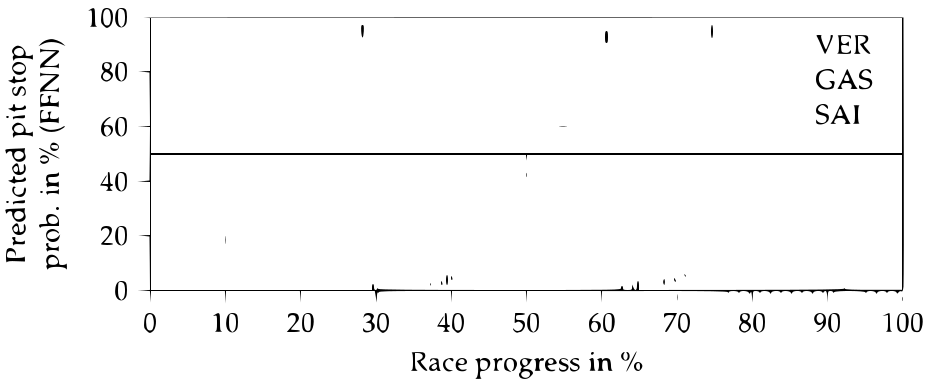
\includegraphics[width=0.7\textwidth]{assets/figures/vse_ffnn.png}
        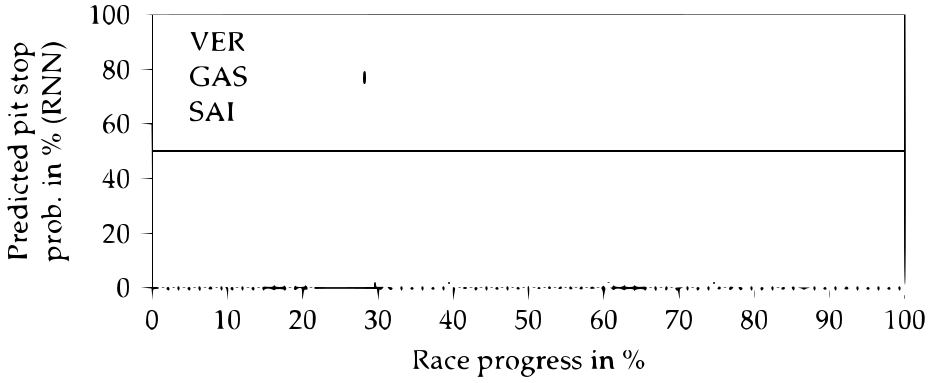
\includegraphics[width=0.7\textwidth]{assets/figures/vse_rnn.png}
        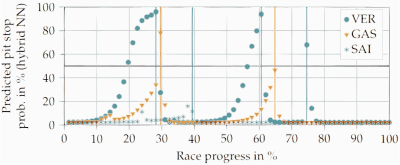
\includegraphics[width=0.7\textwidth]{assets/figures/vse_hnn.png}
        \caption{\label{vse_ffnn}Progression des probabilités d'arrêt au stand pour trois pilotes prédites par le réseau feed-forward, le réseau récurrent et le réseau hybride en utilisant des données du Grand Prix du Brésil 2019, figure repris du papier "Virtual Strategy Engineer: Using Artificial Neural Networks for Making Race Strategy Decisions in Circuit Motorsport"}
    \end{center}
\end{figure}

Les 2 travaux "Tire Changes, Fresh Air, and Yellow Flags: Challenges in Predictive Analytics for Professional Racing" \cite{doi:10.1089/big.2014.0018} et "Real-time decision making in motorsports : analytics for improving professional car race strategy"\cite{phdthesis}
sont des équivalences à notre problématique appliquée au monde de la NASCAR. La NASCAR est une course compétition américaine sur circuits ovales avec des voitures de série modifiées,
dans ce contexte, met davantage l'accent sur les courses en peloton, les dépassements sont plus fréquents et le ravitaillement en carburant est un facteur stratégique majeur.
Ils apportent cependant une formulation différente intéressante, la variable prédite par ses systèmes est le nombre de positions gagnées ou perdues à la suite d'une décision stratégique.

Finalement, on peut noter l'article “Formula-E race strategy development using distributed policy gradient reinforcement learning” de l'université de Cranfield \cite{LIU2021106781} qui utilise une approche de reinforcement learning pour établir une stratégie.
Cet article présente une méthode de développement de stratégies de course dans le contexte du championnat de Formule E, où les voitures ne changent pas de pneus et où la stratégie est davantage liée à l'économie de la batterie.
Cependant, bien que le contexte soit différent de celui proposé dans ce projet et que l'approche reinforcement learning nécessite une simulation précise, la méthode utilisée reste intéressante à noter.

\section{Méthodologie}
La méthodologie adoptée pour cette thèse comprendra les étapes suivantes. Tout d'abord, une analyse approfondie des données disponibles sera réalisée afin d'acquérir une connaissance approfondie de la problématique étudiée.
Ensuite, plusieurs formulations du problème, modèles et méthodes seront explorés à travers des expérimentations.
Les performances respectives de ces approches seront mesurées à l'aide de différentes métriques pour confirmer leur adéquation avec l'objectif fixé.